%%=============================================================================
%% Inleiding
%%=============================================================================

\chapter{\IfLanguageName{dutch}{Inleiding}{Introduction}}
\label{ch:inleiding}


\section{Context}

De dag van vandaag worden bij bijna geboren met technologie in onze handen. Kinderen krijgen al een gsm voor ze twaalf jaar oud zijn. Technologie wordt steeds slimmer en slimmer. We gebruiken overal een app voor, van overschrijvingen tot weersvoorspellingen. Meer en meer komt de mens in contact met technologie. 

Met een wereld vol tech is het dus belangrijk om kinderen te laten leren over computers. We moeten volgens het onderwijsdecreet mensen creëren die kritischer kunnen omgaan met technologie. Logisch dat leerlingen vroeger en vroeger leren programmeren. Zo maakt Vlaams minister Ben Weyts\footnote{Vlaams minister van Onderwijs, sport, Dierenwelzijn en Vlaamse Rand} 375 miljoen euro uit voor digitale innovatie in het onderwijs. Hiermee wil het een laptop voor elke leerling. Dit is niet alleen kostelijk, maar misschien ook niet de beste optie. Zo kun je niet zomaar een laptop in de schoot werpen van elke student en dit digitale innovatie noemen.

Dit onderzoek vraagt zicht af als er andere opties bestaan om te leren programmeren. Zo stelt het een alternatief voor: een single board computer. Een single board computer is, zoals de naam impliceert, een computer waarvan alle onderdelen op een enkele printplaat staan.
Deze onderdelen voor het maken van een functionele computer bestaan uit het volgende:
\begin{itemize}
    \item Microprocessor
    \item Geheugen
    \item Input en ouput poorten
\end{itemize} 
Deze 'naakte computer' is niet veel groter dan een creditkaart en is dus een volwaardige computer: geen nood aan een externe pc! Figuur \ref{fig:raspberryPi1} toont een voorbeeld van een single board computer: de Raspberry Pi 4B. 

\begin{figure}
    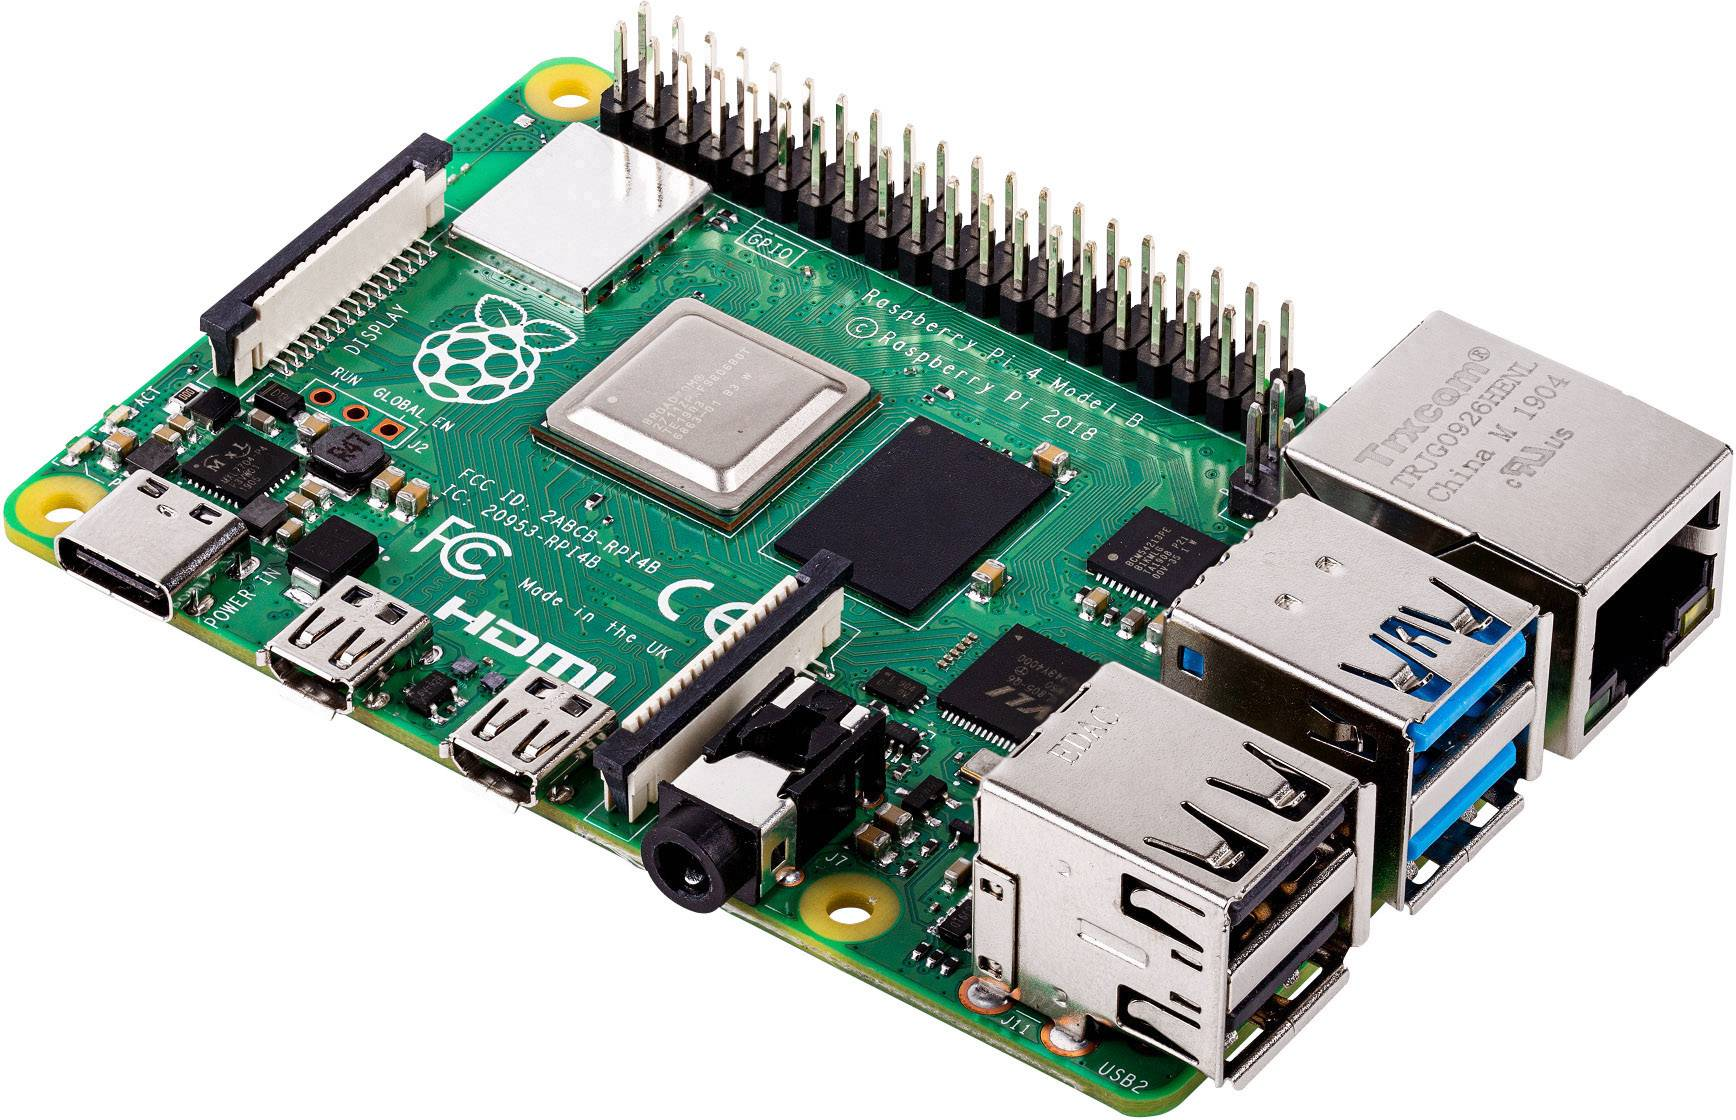
\includegraphics[width=\linewidth]{raspberryPi1}
    \caption{de Raspberry Pi 4B}
    \label{fig:raspberryPi1}
\end{figure}

Aangezien dit een volwaardige computer is, kan dit zelfs gebruikt worden als personal computer (pc). Zo zou een leerkracht een volledige les kunnen geven door enkel gebruik te maken van een minicomputer. Ook kan het de leerlingen een kijkje geven in de wereld van computers. Tenslotte zou dit een goedkopere alternatief zijn dan een laptop, aangezien de meeste single board computers niet veel duurder zijn dan 50 euro.
In dit onderzoek zullen we verder kijken hoe een single board computer kan gebruikt worden in de les:

\section{\IfLanguageName{dutch}{Probleemstelling}{Problem Statement}}
\label{sec:probleemstelling}

Dit onderzoek bekijkt een alternatief voor de laptop in de klas: een single board computer. We bakenen onze doelgroep af tot de leerlingen van de eerste graad secundair onderwijs. Deze bachelorproef zou dus een meerwaarde kunnen geven aan scholen die hun kinderen willen leren programmeren. Ook zou dit een goedkopere optie zijn. 

Om specifieker te zijn, kan het leerkrachten van de eerste graad helpen de eindtermen over digitale competentie en mediawijsheid om te vormen naar praktische voorbeelden. Met behulp van een single board computer zouden leerkrachten ook leerlingen kunnen bijleren over de wereld van computers.

\section{\IfLanguageName{dutch}{Onderzoeksvraag}{Research question}}
\label{sec:onderzoeksvraag}

\begin{itemize}
    \item Welke eindtermen zijn noodzakelijk voor een programmeerles in het onderwijs?
    \item Welke single board computers worden vandaag al ingezet in het onderwijs?
    \item Welke programmeertaal is optimaal voor het leren programmeren op een middelbaar onderwijs niveau?
    \item Welke voorbeelden van educatieve toepassingen bestaan al voor single board computers?
    \item Hoe voer je een educatieve toepassing van mini-computers uit?
    \item Wat zijn de voordelen van single board computers tegenover klassieke computers?
    \item Wat zijn de zwakke punten van single board computers?
\end{itemize}

\section{\IfLanguageName{dutch}{Onderzoeksdoelstelling}{Research objective}}
\label{sec:onderzoeksdoelstelling}

Het doel van deze onderzoeksopdracht is het uitwerken van een project op een singleboard computer, met de optimale programmeertaal. Deze programmeertaal moet afgestemd zijn op het niveau van de leerlingen van de eerste graad secundair. Ook moet de single board computer makkelijk zijn om te gebruiken en goedkoop in aankoopprijs zijn. Tenslotte moeten alle noodzakelijke eindtermen rond programmeren in de eerste graad secundair onderwijs aanwezig zijn.

We zullen dit uitwerken aan de hand van een lesvoorbereiding die stap voor stap het proces uitlegd. Hierbij zullen duidelijk de noodzakelijke doelstellingen opgesomd worden en toegepast in het project. Ook moet het technische steun geven aan de leerkracht om de vlotheid van de les te bewaren.

\section{\IfLanguageName{dutch}{Opzet van deze bachelorproef}{Structure of this bachelor thesis}}
\label{sec:opzet-bachelorproef}

% Het is gebruikelijk aan het einde van de inleiding een overzicht te
% geven van de opbouw van de rest van de tekst. Deze sectie bevat al een aanzet
% die je kan aanvullen/aanpassen in functie van je eigen tekst.

De rest van deze bachelorproef is als volgt opgebouwd:

In Hoofdstuk~\ref{ch:stand-van-zaken} wordt een overzicht gegeven van de stand van zaken binnen het onderzoeksdomein, op basis van een literatuurstudie.

In Hoofdstuk~\ref{ch:methodologie} wordt de methodologie toegelicht en worden de gebruikte onderzoekstechnieken besproken om een antwoord te kunnen formuleren op de onderzoeksvragen.

% TODO: Vul hier aan voor je eigen hoofstukken, één of twee zinnen per hoofdstuk

in het Hoofdstuk~\ref{ch:lesvoorbereiding} wordt de uitgewerkte lesvoorbereiding toegelicht en wordt de feedback op deze voorbereiding gepresenteerd.

In Hoofdstuk~\ref{ch:conclusie}, tenslotte, wordt de conclusie gegeven en een antwoord geformuleerd op de onderzoeksvragen. Daarbij wordt ook een aanzet gegeven voor toekomstig onderzoek binnen dit domein.